\subsection{Definition}
This example illustrates the disturbance of the uniform flow in porous media caused by the presence of a fracture. 
%
Consider a 2D infinite horizontal plane of porous media with an embedded fracture. Uniform flow with specific discharge $q_0$ occurs from the left side to the right of the domain. The fracture extends to infinity in the directions normal to the plane. The middle point of the fracture is placed at the center of the plane. 
%
The shape of the fracture is shown in Figure \ref{fig:Hmf_frac}. The fracture has a length of $L$ and is inclined with angle $\beta$. 
The fracture aperture $b$ may vary with positions. In this example, it is assumed that the shape corresponds to that obtained from the normal displacements of the sides of a pressurized crack in an elastic medium. This gives
%
\begin{equation}
b = b_\mathrm{max} \sqrt{1-x'^2}	
\end{equation}
%
where $x'$ is the normalized local coordinate systems. $b_\mathrm{max}$  is the aperture at the center $x'=0$.
%
Assuming the volume of the fracture is sufficiently small as compared to that of porous media, the flow in the porous media can be modeled ignoring the width of the fracture. The flow in the fracture is assumed to be laminar along the fracture surface. Hydraulic conductivity of the fracture is constant and independent of the aperture variation. The pressure variation across the fracture is neglected.

\begin{figure}[htb]
\centering
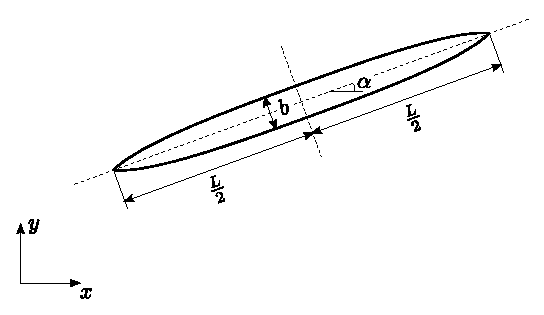
\includegraphics[width=0.5\textwidth]{Chapter5/figure/Hmf_uniform_flow_frac}
\caption{Fracture geometry}
\label{fig:Hmf_frac}
\end{figure}

\begin{table}[htb]
\centering
\caption{Model parameters}
\begin{tabular*}{0.9\textwidth}{@{\extracolsep{\fill}}llrr}
\hline\noalign{\smallskip}
 Symbol &Parameter& Value & Unit \\ 
\hline\noalign{\smallskip}
$\alpha$ 				&fracture angle  		& 45 									&  $\circ$  \\		
$b_\mathbf{max}$ 	&maximum fracture aperture & $0.05$  & $m$ \\
$L$ 	& fracture length & $2.0$  & $m$ \\
$K_f$ 	&fracture hydraulic conductivity & $1.0\times 10^{-3}$ 	& $m/s$ \\
$K_m$ 	&porous medium hydraulic conductivity & $1.0\times 10^{-5}$ 	& $m/s$ \\
$q_0$ 	&specific discharge & $1.0\times 10^{-4}$ 	& $m/s$ \\
\noalign{\smallskip}\hline
\end{tabular*}
\label{tab:Hmf_parameters}
\end{table}

\subsection{Solution}
\subsubsection{Analytical solution}
Strack \cite{Strack1982} has derived an exact solution for this problem as the potential flow. The obtained complex potential $\Omega$ is given as

\begin{equation}
\Omega = - A \sqrt{(Z-1)(Z+1)} + A Z - \frac{1}{2} q_0 L e^{i \alpha} Z + C	
\end{equation}

\noindent
for the dimensionless variable $Z$ 
%
\begin{equation}
Z = X + i Y = \frac{z-\frac{1}{2}(z_1+z_2)}{\frac{1}{2}(z_2-z_1)}	
\end{equation}
%
with the endpoints of the fracture $z_1$ and $z_2$. $A$ is defined as

\begin{equation}
A = \frac{\frac{1}{2}K_f b_\mathrm{max}}{K_m L + K_f b_\mathrm{max}}	q_0 L \cos \alpha
\end{equation}

\noindent
and $C$ is the integration constant. In this example, the constant is simply considered as zero.


\subsubsection{Numerical solution}
Numerical solution can be obtained by solving steady state liquid flow problem in a hybrid system of a discrete fracture model and continuum model (porous media). The fracture is represented as a 1D hydraulic conduit. The domain is set up in a finite space as a square with length of 10 m as depicted in Figure \ref{fig:Hmf_domain}. 
%
To compare numerical results with the analytical solution, pressure calculated by the analytical solution is utilized as prescribed pressure  at the lateral boundaries, i.e. $p_\mathrm{in}=496465$ Pa and $p_\mathrm{out}=-496465$ Pa. It is assumed that the fracture aperture does not vary with positions and has constant value even at the endpoints, $b=b_\mathrm{max}$.

\begin{figure}[htb]
\centering
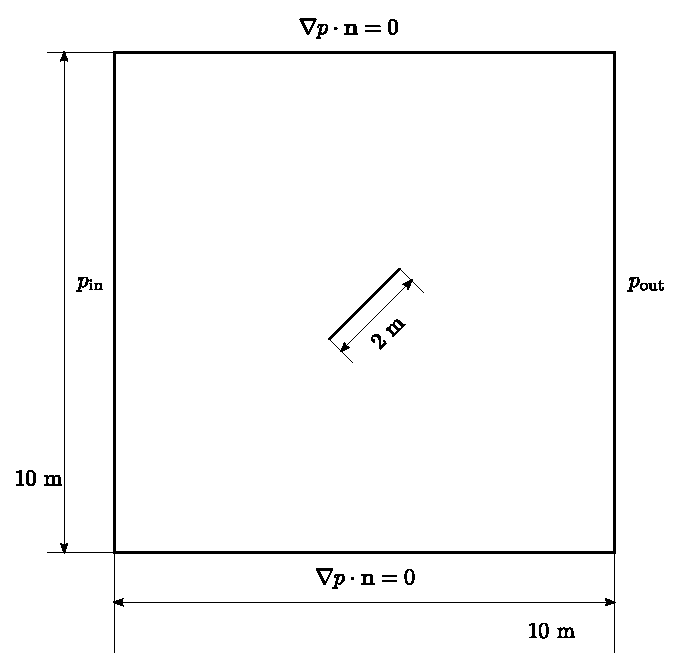
\includegraphics[width=0.7\textwidth]{Chapter5/figure/Hmf_uniform_flow_domain}
\caption{Computational area}
\label{fig:Hmf_domain}
\end{figure}


\subsection{Results}

Pressure distribution obtained by the analytical solution is shown in Figure \ref{fig:Hmf_pressure_dis}. Lateral uniform flow is disturbed in the vicinity of the inclined fracture where the flow is faster than in surrounding porous media. 
%
Figure \ref{fig:Hmf_pressure_cross} presents the pressure profile along a diagonal line from the bottom-left to the top-right. Although the numerical solution adopts the idealized fracture geometry, results show  good agreements between the numerical and the analytical solution. 


\begin{figure}[htb]
\centering
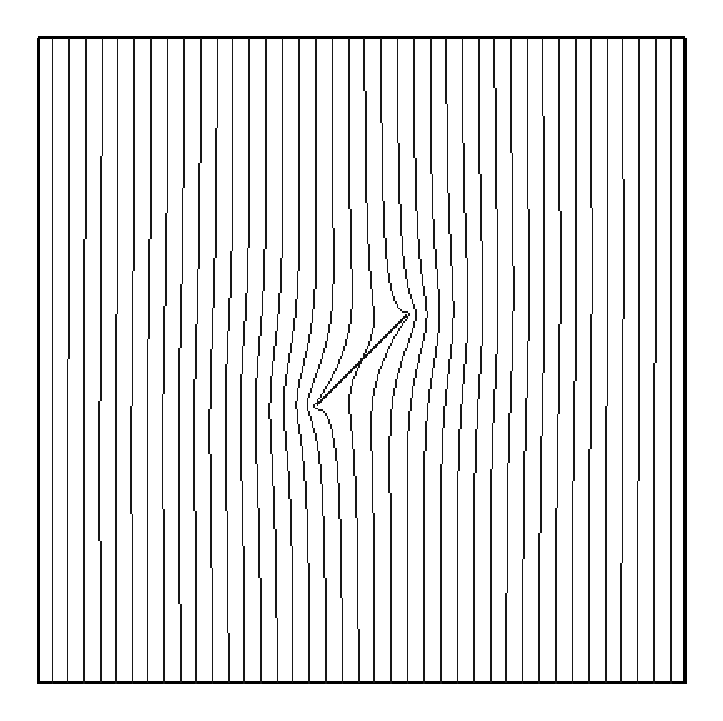
\includegraphics[width=0.5\textwidth]{Chapter5/figure/Hmf_uniform_flow_pressure}
\caption{Pressure distribution obtained by the analytical solution}
\label{fig:Hmf_pressure_dis}
\end{figure}


\begin{figure}[htb]
\centering
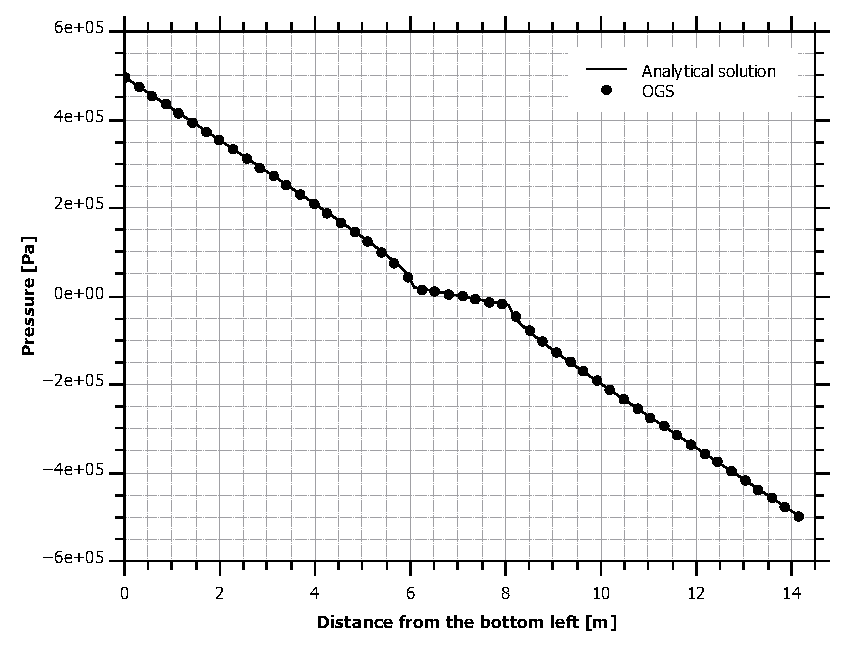
\includegraphics[width=0.8\textwidth]{Chapter5/figure/Hmf_uniform_flow_a45-cross-profile}
\caption{Pressure profile along a diagonal line from the bottom-left to the top-right}
\label{fig:Hmf_pressure_cross}
\end{figure}
